\section{Aproksymacja odpowiedzi skokowej}

Dla odpowiedzi skokowej z wartości mocy grzałki równej 0\% do wartości 30\% dokonano aproksymacji jako człon inercyjny drugiego rzędu z
opóźnieniem o transmitancji  (\ref{transmitance}).

\begin{equation}
   G(s) = \frac{K}{(sT_1 + 1)(sT_2 + 1)}e^{- T_d} s
   \label{transmitance}
\end{equation}

Uzyskaną odpowiedź skokową przekształcono do znormalizowanej postaci.
\begin{equation}
    s_i = (Y_i - Y_{pp})/30
\end{equation}

Zaimplementowano funkcję \texttt{simulation.m} symulującą wartości odpowiedzi skokowej dla takiego członu oraz wyznaczjącą wskaźnik jakości aproksymacji w stosunku do podanej odpowiedzi skokowej. Wskaźnikiem jakości była suma kwadratów róznic pomiędzy wartością oczekiwaną, a uzyskaną. Paramterami symulacji były: $T_1, T_2, K, T_d$.
Wcelu dobrania optymalnych parametrów aproksymacji odpowiedzi skokowej wykonano serię przeszukiwań przestrzeni parametrów $T_1, T_2, K$ dla parametru $T_d$ przyjmującego kolejno wartości od 1 do 30. Z serii tej wybrano zestaw parametrów dla których wskaźnik jakości był najmniejszy.
Uzyskane paramtery to: $T_1 = \num{69.880}, T_2 = \num{11.765}, K = \num{0.295}, T_d = 14$. Uzyskano wskaźnik jakości aproksymacji $E = \num{0.0012}$. Na rysunku \ref{aprox} znajduje się zestawienie pobranej odpowiedzi skokowej i aproksymowanej.

\begin{figure}
\label{aprox}
\centering
\caption{Odpowiedź skokowa obiektu oraz odpowiedź aproksymowana}
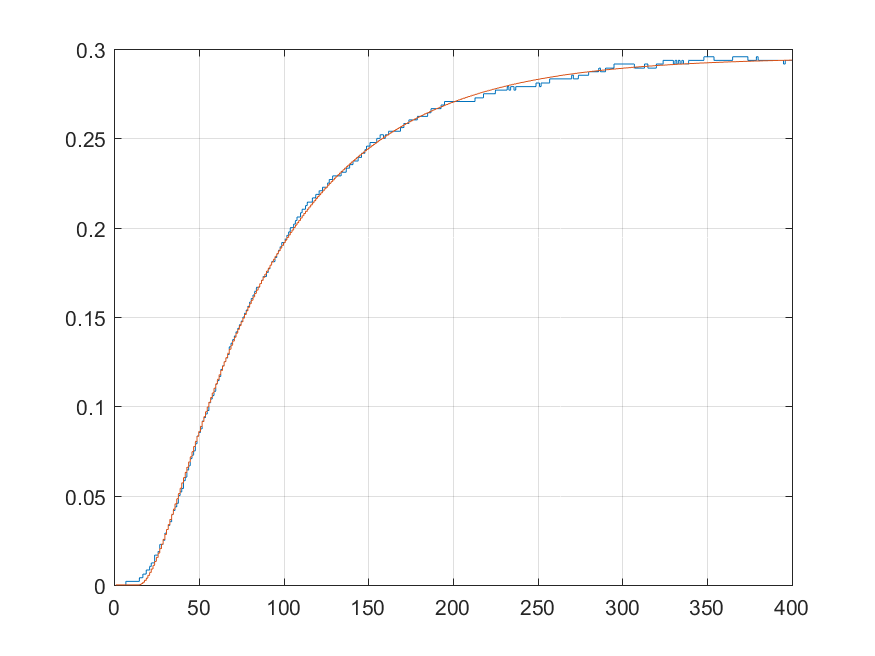
\includegraphics{aproximation.png}
\end{figure}